\documentclass[11pt]{article}

    \usepackage[breakable]{tcolorbox}
    \usepackage{parskip} % Stop auto-indenting (to mimic markdown behaviour)
    
    \usepackage{iftex}
    \ifPDFTeX
    	\usepackage[T1]{fontenc}
    	\usepackage{mathpazo}
    \else
    	\usepackage{fontspec}
    \fi

    % Basic figure setup, for now with no caption control since it's done
    % automatically by Pandoc (which extracts ![](path) syntax from Markdown).
    \usepackage{graphicx}
    % Maintain compatibility with old templates. Remove in nbconvert 6.0
    \let\Oldincludegraphics\includegraphics
    % Ensure that by default, figures have no caption (until we provide a
    % proper Figure object with a Caption API and a way to capture that
    % in the conversion process - todo).
    \usepackage{caption}
    \DeclareCaptionFormat{nocaption}{}
    \captionsetup{format=nocaption,aboveskip=0pt,belowskip=0pt}

    \usepackage[Export]{adjustbox} % Used to constrain images to a maximum size
    \adjustboxset{max size={0.9\linewidth}{0.9\paperheight}}
    \usepackage{float}
    \usepackage{graphicx}
    \floatplacement{figure}{H} % forces figures to be placed at the correct location
    \usepackage{xcolor} % Allow colors to be defined
    \usepackage{enumerate} % Needed for markdown enumerations to work
    \usepackage{geometry} % Used to adjust the document margins
    \usepackage{amsmath} % Equations
    \usepackage{amssymb} % Equations
    \usepackage{textcomp} % defines textquotesingle
    % Hack from http://tex.stackexchange.com/a/47451/13684:
    \AtBeginDocument{%
        \def\PYZsq{\textquotesingle}% Upright quotes in Pygmentized code
    }
    \usepackage{upquote} % Upright quotes for verbatim code
    \usepackage{eurosym} % defines \euro
    \usepackage[mathletters]{ucs} % Extended unicode (utf-8) support
    \usepackage{fancyvrb} % verbatim replacement that allows latex
    \usepackage{grffile} % extends the file name processing of package graphics 
                         % to support a larger range
    \makeatletter % fix for grffile with XeLaTeX
    \def\Gread@@xetex#1{%
      \IfFileExists{"\Gin@base".bb}%
      {\Gread@eps{\Gin@base.bb}}%
      {\Gread@@xetex@aux#1}%
    }
    \makeatother

    % The hyperref package gives us a pdf with properly built
    % internal navigation ('pdf bookmarks' for the table of contents,
    % internal cross-reference links, web links for URLs, etc.)
    \usepackage{hyperref}
    % The default LaTeX title has an obnoxious amount of whitespace. By default,
    % titling removes some of it. It also provides customization options.
    \usepackage{titling}
    \usepackage{longtable} % longtable support required by pandoc >1.10
    \usepackage{booktabs}  % table support for pandoc > 1.12.2
    \usepackage[inline]{enumitem} % IRkernel/repr support (it uses the enumerate* environment)
    \usepackage[normalem]{ulem} % ulem is needed to support strikethroughs (\sout)
                                % normalem makes italics be italics, not underlines
    \usepackage{mathrsfs}
    

    
    % Colors for the hyperref package
    \definecolor{urlcolor}{rgb}{0,.145,.698}
    \definecolor{linkcolor}{rgb}{.71,0.21,0.01}
    \definecolor{citecolor}{rgb}{.12,.54,.11}

    % ANSI colors
    \definecolor{ansi-black}{HTML}{3E424D}
    \definecolor{ansi-black-intense}{HTML}{282C36}
    \definecolor{ansi-red}{HTML}{E75C58}
    \definecolor{ansi-red-intense}{HTML}{B22B31}
    \definecolor{ansi-green}{HTML}{00A250}
    \definecolor{ansi-green-intense}{HTML}{007427}
    \definecolor{ansi-yellow}{HTML}{DDB62B}
    \definecolor{ansi-yellow-intense}{HTML}{B27D12}
    \definecolor{ansi-blue}{HTML}{208FFB}
    \definecolor{ansi-blue-intense}{HTML}{0065CA}
    \definecolor{ansi-magenta}{HTML}{D160C4}
    \definecolor{ansi-magenta-intense}{HTML}{A03196}
    \definecolor{ansi-cyan}{HTML}{60C6C8}
    \definecolor{ansi-cyan-intense}{HTML}{258F8F}
    \definecolor{ansi-white}{HTML}{C5C1B4}
    \definecolor{ansi-white-intense}{HTML}{A1A6B2}
    \definecolor{ansi-default-inverse-fg}{HTML}{FFFFFF}
    \definecolor{ansi-default-inverse-bg}{HTML}{000000}

    % commands and environments needed by pandoc snippets
    % extracted from the output of `pandoc -s`
    \providecommand{\tightlist}{%
      \setlength{\itemsep}{0pt}\setlength{\parskip}{0pt}}
    \DefineVerbatimEnvironment{Highlighting}{Verbatim}{commandchars=\\\{\}}
    % Add ',fontsize=\small' for more characters per line
    \newenvironment{Shaded}{}{}
    \newcommand{\KeywordTok}[1]{\textcolor[rgb]{0.00,0.44,0.13}{\textbf{{#1}}}}
    \newcommand{\DataTypeTok}[1]{\textcolor[rgb]{0.56,0.13,0.00}{{#1}}}
    \newcommand{\DecValTok}[1]{\textcolor[rgb]{0.25,0.63,0.44}{{#1}}}
    \newcommand{\BaseNTok}[1]{\textcolor[rgb]{0.25,0.63,0.44}{{#1}}}
    \newcommand{\FloatTok}[1]{\textcolor[rgb]{0.25,0.63,0.44}{{#1}}}
    \newcommand{\CharTok}[1]{\textcolor[rgb]{0.25,0.44,0.63}{{#1}}}
    \newcommand{\StringTok}[1]{\textcolor[rgb]{0.25,0.44,0.63}{{#1}}}
    \newcommand{\CommentTok}[1]{\textcolor[rgb]{0.38,0.63,0.69}{\textit{{#1}}}}
    \newcommand{\OtherTok}[1]{\textcolor[rgb]{0.00,0.44,0.13}{{#1}}}
    \newcommand{\AlertTok}[1]{\textcolor[rgb]{1.00,0.00,0.00}{\textbf{{#1}}}}
    \newcommand{\FunctionTok}[1]{\textcolor[rgb]{0.02,0.16,0.49}{{#1}}}
    \newcommand{\RegionMarkerTok}[1]{{#1}}
    \newcommand{\ErrorTok}[1]{\textcolor[rgb]{1.00,0.00,0.00}{\textbf{{#1}}}}
    \newcommand{\NormalTok}[1]{{#1}}
    
    % Additional commands for more recent versions of Pandoc
    \newcommand{\ConstantTok}[1]{\textcolor[rgb]{0.53,0.00,0.00}{{#1}}}
    \newcommand{\SpecialCharTok}[1]{\textcolor[rgb]{0.25,0.44,0.63}{{#1}}}
    \newcommand{\VerbatimStringTok}[1]{\textcolor[rgb]{0.25,0.44,0.63}{{#1}}}
    \newcommand{\SpecialStringTok}[1]{\textcolor[rgb]{0.73,0.40,0.53}{{#1}}}
    \newcommand{\ImportTok}[1]{{#1}}
    \newcommand{\DocumentationTok}[1]{\textcolor[rgb]{0.73,0.13,0.13}{\textit{{#1}}}}
    \newcommand{\AnnotationTok}[1]{\textcolor[rgb]{0.38,0.63,0.69}{\textbf{\textit{{#1}}}}}
    \newcommand{\CommentVarTok}[1]{\textcolor[rgb]{0.38,0.63,0.69}{\textbf{\textit{{#1}}}}}
    \newcommand{\VariableTok}[1]{\textcolor[rgb]{0.10,0.09,0.49}{{#1}}}
    \newcommand{\ControlFlowTok}[1]{\textcolor[rgb]{0.00,0.44,0.13}{\textbf{{#1}}}}
    \newcommand{\OperatorTok}[1]{\textcolor[rgb]{0.40,0.40,0.40}{{#1}}}
    \newcommand{\BuiltInTok}[1]{{#1}}
    \newcommand{\ExtensionTok}[1]{{#1}}
    \newcommand{\PreprocessorTok}[1]{\textcolor[rgb]{0.74,0.48,0.00}{{#1}}}
    \newcommand{\AttributeTok}[1]{\textcolor[rgb]{0.49,0.56,0.16}{{#1}}}
    \newcommand{\InformationTok}[1]{\textcolor[rgb]{0.38,0.63,0.69}{\textbf{\textit{{#1}}}}}
    \newcommand{\WarningTok}[1]{\textcolor[rgb]{0.38,0.63,0.69}{\textbf{\textit{{#1}}}}}
    
    
    % Define a nice break command that doesn't care if a line doesn't already
    % exist.
    \def\br{\hspace*{\fill} \\* }
    % Math Jax compatibility definitions
    \def\gt{>}
    \def\lt{<}
    \let\Oldtex\TeX
    \let\Oldlatex\LaTeX
    \renewcommand{\TeX}{\textrm{\Oldtex}}
    \renewcommand{\LaTeX}{\textrm{\Oldlatex}}
    % Document parameters
    % Document title
    \title{janakparajuli\_api\_request\_deckgl}
    
    
    
    
    
% Pygments definitions
\makeatletter
\def\PY@reset{\let\PY@it=\relax \let\PY@bf=\relax%
    \let\PY@ul=\relax \let\PY@tc=\relax%
    \let\PY@bc=\relax \let\PY@ff=\relax}
\def\PY@tok#1{\csname PY@tok@#1\endcsname}
\def\PY@toks#1+{\ifx\relax#1\empty\else%
    \PY@tok{#1}\expandafter\PY@toks\fi}
\def\PY@do#1{\PY@bc{\PY@tc{\PY@ul{%
    \PY@it{\PY@bf{\PY@ff{#1}}}}}}}
\def\PY#1#2{\PY@reset\PY@toks#1+\relax+\PY@do{#2}}

\expandafter\def\csname PY@tok@w\endcsname{\def\PY@tc##1{\textcolor[rgb]{0.73,0.73,0.73}{##1}}}
\expandafter\def\csname PY@tok@c\endcsname{\let\PY@it=\textit\def\PY@tc##1{\textcolor[rgb]{0.25,0.50,0.50}{##1}}}
\expandafter\def\csname PY@tok@cp\endcsname{\def\PY@tc##1{\textcolor[rgb]{0.74,0.48,0.00}{##1}}}
\expandafter\def\csname PY@tok@k\endcsname{\let\PY@bf=\textbf\def\PY@tc##1{\textcolor[rgb]{0.00,0.50,0.00}{##1}}}
\expandafter\def\csname PY@tok@kp\endcsname{\def\PY@tc##1{\textcolor[rgb]{0.00,0.50,0.00}{##1}}}
\expandafter\def\csname PY@tok@kt\endcsname{\def\PY@tc##1{\textcolor[rgb]{0.69,0.00,0.25}{##1}}}
\expandafter\def\csname PY@tok@o\endcsname{\def\PY@tc##1{\textcolor[rgb]{0.40,0.40,0.40}{##1}}}
\expandafter\def\csname PY@tok@ow\endcsname{\let\PY@bf=\textbf\def\PY@tc##1{\textcolor[rgb]{0.67,0.13,1.00}{##1}}}
\expandafter\def\csname PY@tok@nb\endcsname{\def\PY@tc##1{\textcolor[rgb]{0.00,0.50,0.00}{##1}}}
\expandafter\def\csname PY@tok@nf\endcsname{\def\PY@tc##1{\textcolor[rgb]{0.00,0.00,1.00}{##1}}}
\expandafter\def\csname PY@tok@nc\endcsname{\let\PY@bf=\textbf\def\PY@tc##1{\textcolor[rgb]{0.00,0.00,1.00}{##1}}}
\expandafter\def\csname PY@tok@nn\endcsname{\let\PY@bf=\textbf\def\PY@tc##1{\textcolor[rgb]{0.00,0.00,1.00}{##1}}}
\expandafter\def\csname PY@tok@ne\endcsname{\let\PY@bf=\textbf\def\PY@tc##1{\textcolor[rgb]{0.82,0.25,0.23}{##1}}}
\expandafter\def\csname PY@tok@nv\endcsname{\def\PY@tc##1{\textcolor[rgb]{0.10,0.09,0.49}{##1}}}
\expandafter\def\csname PY@tok@no\endcsname{\def\PY@tc##1{\textcolor[rgb]{0.53,0.00,0.00}{##1}}}
\expandafter\def\csname PY@tok@nl\endcsname{\def\PY@tc##1{\textcolor[rgb]{0.63,0.63,0.00}{##1}}}
\expandafter\def\csname PY@tok@ni\endcsname{\let\PY@bf=\textbf\def\PY@tc##1{\textcolor[rgb]{0.60,0.60,0.60}{##1}}}
\expandafter\def\csname PY@tok@na\endcsname{\def\PY@tc##1{\textcolor[rgb]{0.49,0.56,0.16}{##1}}}
\expandafter\def\csname PY@tok@nt\endcsname{\let\PY@bf=\textbf\def\PY@tc##1{\textcolor[rgb]{0.00,0.50,0.00}{##1}}}
\expandafter\def\csname PY@tok@nd\endcsname{\def\PY@tc##1{\textcolor[rgb]{0.67,0.13,1.00}{##1}}}
\expandafter\def\csname PY@tok@s\endcsname{\def\PY@tc##1{\textcolor[rgb]{0.73,0.13,0.13}{##1}}}
\expandafter\def\csname PY@tok@sd\endcsname{\let\PY@it=\textit\def\PY@tc##1{\textcolor[rgb]{0.73,0.13,0.13}{##1}}}
\expandafter\def\csname PY@tok@si\endcsname{\let\PY@bf=\textbf\def\PY@tc##1{\textcolor[rgb]{0.73,0.40,0.53}{##1}}}
\expandafter\def\csname PY@tok@se\endcsname{\let\PY@bf=\textbf\def\PY@tc##1{\textcolor[rgb]{0.73,0.40,0.13}{##1}}}
\expandafter\def\csname PY@tok@sr\endcsname{\def\PY@tc##1{\textcolor[rgb]{0.73,0.40,0.53}{##1}}}
\expandafter\def\csname PY@tok@ss\endcsname{\def\PY@tc##1{\textcolor[rgb]{0.10,0.09,0.49}{##1}}}
\expandafter\def\csname PY@tok@sx\endcsname{\def\PY@tc##1{\textcolor[rgb]{0.00,0.50,0.00}{##1}}}
\expandafter\def\csname PY@tok@m\endcsname{\def\PY@tc##1{\textcolor[rgb]{0.40,0.40,0.40}{##1}}}
\expandafter\def\csname PY@tok@gh\endcsname{\let\PY@bf=\textbf\def\PY@tc##1{\textcolor[rgb]{0.00,0.00,0.50}{##1}}}
\expandafter\def\csname PY@tok@gu\endcsname{\let\PY@bf=\textbf\def\PY@tc##1{\textcolor[rgb]{0.50,0.00,0.50}{##1}}}
\expandafter\def\csname PY@tok@gd\endcsname{\def\PY@tc##1{\textcolor[rgb]{0.63,0.00,0.00}{##1}}}
\expandafter\def\csname PY@tok@gi\endcsname{\def\PY@tc##1{\textcolor[rgb]{0.00,0.63,0.00}{##1}}}
\expandafter\def\csname PY@tok@gr\endcsname{\def\PY@tc##1{\textcolor[rgb]{1.00,0.00,0.00}{##1}}}
\expandafter\def\csname PY@tok@ge\endcsname{\let\PY@it=\textit}
\expandafter\def\csname PY@tok@gs\endcsname{\let\PY@bf=\textbf}
\expandafter\def\csname PY@tok@gp\endcsname{\let\PY@bf=\textbf\def\PY@tc##1{\textcolor[rgb]{0.00,0.00,0.50}{##1}}}
\expandafter\def\csname PY@tok@go\endcsname{\def\PY@tc##1{\textcolor[rgb]{0.53,0.53,0.53}{##1}}}
\expandafter\def\csname PY@tok@gt\endcsname{\def\PY@tc##1{\textcolor[rgb]{0.00,0.27,0.87}{##1}}}
\expandafter\def\csname PY@tok@err\endcsname{\def\PY@bc##1{\setlength{\fboxsep}{0pt}\fcolorbox[rgb]{1.00,0.00,0.00}{1,1,1}{\strut ##1}}}
\expandafter\def\csname PY@tok@kc\endcsname{\let\PY@bf=\textbf\def\PY@tc##1{\textcolor[rgb]{0.00,0.50,0.00}{##1}}}
\expandafter\def\csname PY@tok@kd\endcsname{\let\PY@bf=\textbf\def\PY@tc##1{\textcolor[rgb]{0.00,0.50,0.00}{##1}}}
\expandafter\def\csname PY@tok@kn\endcsname{\let\PY@bf=\textbf\def\PY@tc##1{\textcolor[rgb]{0.00,0.50,0.00}{##1}}}
\expandafter\def\csname PY@tok@kr\endcsname{\let\PY@bf=\textbf\def\PY@tc##1{\textcolor[rgb]{0.00,0.50,0.00}{##1}}}
\expandafter\def\csname PY@tok@bp\endcsname{\def\PY@tc##1{\textcolor[rgb]{0.00,0.50,0.00}{##1}}}
\expandafter\def\csname PY@tok@fm\endcsname{\def\PY@tc##1{\textcolor[rgb]{0.00,0.00,1.00}{##1}}}
\expandafter\def\csname PY@tok@vc\endcsname{\def\PY@tc##1{\textcolor[rgb]{0.10,0.09,0.49}{##1}}}
\expandafter\def\csname PY@tok@vg\endcsname{\def\PY@tc##1{\textcolor[rgb]{0.10,0.09,0.49}{##1}}}
\expandafter\def\csname PY@tok@vi\endcsname{\def\PY@tc##1{\textcolor[rgb]{0.10,0.09,0.49}{##1}}}
\expandafter\def\csname PY@tok@vm\endcsname{\def\PY@tc##1{\textcolor[rgb]{0.10,0.09,0.49}{##1}}}
\expandafter\def\csname PY@tok@sa\endcsname{\def\PY@tc##1{\textcolor[rgb]{0.73,0.13,0.13}{##1}}}
\expandafter\def\csname PY@tok@sb\endcsname{\def\PY@tc##1{\textcolor[rgb]{0.73,0.13,0.13}{##1}}}
\expandafter\def\csname PY@tok@sc\endcsname{\def\PY@tc##1{\textcolor[rgb]{0.73,0.13,0.13}{##1}}}
\expandafter\def\csname PY@tok@dl\endcsname{\def\PY@tc##1{\textcolor[rgb]{0.73,0.13,0.13}{##1}}}
\expandafter\def\csname PY@tok@s2\endcsname{\def\PY@tc##1{\textcolor[rgb]{0.73,0.13,0.13}{##1}}}
\expandafter\def\csname PY@tok@sh\endcsname{\def\PY@tc##1{\textcolor[rgb]{0.73,0.13,0.13}{##1}}}
\expandafter\def\csname PY@tok@s1\endcsname{\def\PY@tc##1{\textcolor[rgb]{0.73,0.13,0.13}{##1}}}
\expandafter\def\csname PY@tok@mb\endcsname{\def\PY@tc##1{\textcolor[rgb]{0.40,0.40,0.40}{##1}}}
\expandafter\def\csname PY@tok@mf\endcsname{\def\PY@tc##1{\textcolor[rgb]{0.40,0.40,0.40}{##1}}}
\expandafter\def\csname PY@tok@mh\endcsname{\def\PY@tc##1{\textcolor[rgb]{0.40,0.40,0.40}{##1}}}
\expandafter\def\csname PY@tok@mi\endcsname{\def\PY@tc##1{\textcolor[rgb]{0.40,0.40,0.40}{##1}}}
\expandafter\def\csname PY@tok@il\endcsname{\def\PY@tc##1{\textcolor[rgb]{0.40,0.40,0.40}{##1}}}
\expandafter\def\csname PY@tok@mo\endcsname{\def\PY@tc##1{\textcolor[rgb]{0.40,0.40,0.40}{##1}}}
\expandafter\def\csname PY@tok@ch\endcsname{\let\PY@it=\textit\def\PY@tc##1{\textcolor[rgb]{0.25,0.50,0.50}{##1}}}
\expandafter\def\csname PY@tok@cm\endcsname{\let\PY@it=\textit\def\PY@tc##1{\textcolor[rgb]{0.25,0.50,0.50}{##1}}}
\expandafter\def\csname PY@tok@cpf\endcsname{\let\PY@it=\textit\def\PY@tc##1{\textcolor[rgb]{0.25,0.50,0.50}{##1}}}
\expandafter\def\csname PY@tok@c1\endcsname{\let\PY@it=\textit\def\PY@tc##1{\textcolor[rgb]{0.25,0.50,0.50}{##1}}}
\expandafter\def\csname PY@tok@cs\endcsname{\let\PY@it=\textit\def\PY@tc##1{\textcolor[rgb]{0.25,0.50,0.50}{##1}}}

\def\PYZbs{\char`\\}
\def\PYZus{\char`\_}
\def\PYZob{\char`\{}
\def\PYZcb{\char`\}}
\def\PYZca{\char`\^}
\def\PYZam{\char`\&}
\def\PYZlt{\char`\<}
\def\PYZgt{\char`\>}
\def\PYZsh{\char`\#}
\def\PYZpc{\char`\%}
\def\PYZdl{\char`\$}
\def\PYZhy{\char`\-}
\def\PYZsq{\char`\'}
\def\PYZdq{\char`\"}
\def\PYZti{\char`\~}
% for compatibility with earlier versions
\def\PYZat{@}
\def\PYZlb{[}
\def\PYZrb{]}
\makeatother


    % For linebreaks inside Verbatim environment from package fancyvrb. 
    \makeatletter
        \newbox\Wrappedcontinuationbox 
        \newbox\Wrappedvisiblespacebox 
        \newcommand*\Wrappedvisiblespace {\textcolor{red}{\textvisiblespace}} 
        \newcommand*\Wrappedcontinuationsymbol {\textcolor{red}{\llap{\tiny$\m@th\hookrightarrow$}}} 
        \newcommand*\Wrappedcontinuationindent {3ex } 
        \newcommand*\Wrappedafterbreak {\kern\Wrappedcontinuationindent\copy\Wrappedcontinuationbox} 
        % Take advantage of the already applied Pygments mark-up to insert 
        % potential linebreaks for TeX processing. 
        %        {, <, #, %, $, ' and ": go to next line. 
        %        _, }, ^, &, >, - and ~: stay at end of broken line. 
        % Use of \textquotesingle for straight quote. 
        \newcommand*\Wrappedbreaksatspecials {% 
            \def\PYGZus{\discretionary{\char`\_}{\Wrappedafterbreak}{\char`\_}}% 
            \def\PYGZob{\discretionary{}{\Wrappedafterbreak\char`\{}{\char`\{}}% 
            \def\PYGZcb{\discretionary{\char`\}}{\Wrappedafterbreak}{\char`\}}}% 
            \def\PYGZca{\discretionary{\char`\^}{\Wrappedafterbreak}{\char`\^}}% 
            \def\PYGZam{\discretionary{\char`\&}{\Wrappedafterbreak}{\char`\&}}% 
            \def\PYGZlt{\discretionary{}{\Wrappedafterbreak\char`\<}{\char`\<}}% 
            \def\PYGZgt{\discretionary{\char`\>}{\Wrappedafterbreak}{\char`\>}}% 
            \def\PYGZsh{\discretionary{}{\Wrappedafterbreak\char`\#}{\char`\#}}% 
            \def\PYGZpc{\discretionary{}{\Wrappedafterbreak\char`\%}{\char`\%}}% 
            \def\PYGZdl{\discretionary{}{\Wrappedafterbreak\char`\$}{\char`\$}}% 
            \def\PYGZhy{\discretionary{\char`\-}{\Wrappedafterbreak}{\char`\-}}% 
            \def\PYGZsq{\discretionary{}{\Wrappedafterbreak\textquotesingle}{\textquotesingle}}% 
            \def\PYGZdq{\discretionary{}{\Wrappedafterbreak\char`\"}{\char`\"}}% 
            \def\PYGZti{\discretionary{\char`\~}{\Wrappedafterbreak}{\char`\~}}% 
        } 
        % Some characters . , ; ? ! / are not pygmentized. 
        % This macro makes them "active" and they will insert potential linebreaks 
        \newcommand*\Wrappedbreaksatpunct {% 
            \lccode`\~`\.\lowercase{\def~}{\discretionary{\hbox{\char`\.}}{\Wrappedafterbreak}{\hbox{\char`\.}}}% 
            \lccode`\~`\,\lowercase{\def~}{\discretionary{\hbox{\char`\,}}{\Wrappedafterbreak}{\hbox{\char`\,}}}% 
            \lccode`\~`\;\lowercase{\def~}{\discretionary{\hbox{\char`\;}}{\Wrappedafterbreak}{\hbox{\char`\;}}}% 
            \lccode`\~`\:\lowercase{\def~}{\discretionary{\hbox{\char`\:}}{\Wrappedafterbreak}{\hbox{\char`\:}}}% 
            \lccode`\~`\?\lowercase{\def~}{\discretionary{\hbox{\char`\?}}{\Wrappedafterbreak}{\hbox{\char`\?}}}% 
            \lccode`\~`\!\lowercase{\def~}{\discretionary{\hbox{\char`\!}}{\Wrappedafterbreak}{\hbox{\char`\!}}}% 
            \lccode`\~`\/\lowercase{\def~}{\discretionary{\hbox{\char`\/}}{\Wrappedafterbreak}{\hbox{\char`\/}}}% 
            \catcode`\.\active
            \catcode`\,\active 
            \catcode`\;\active
            \catcode`\:\active
            \catcode`\?\active
            \catcode`\!\active
            \catcode`\/\active 
            \lccode`\~`\~ 	
        }
    \makeatother

    \let\OriginalVerbatim=\Verbatim
    \makeatletter
    \renewcommand{\Verbatim}[1][1]{%
        %\parskip\z@skip
        \sbox\Wrappedcontinuationbox {\Wrappedcontinuationsymbol}%
        \sbox\Wrappedvisiblespacebox {\FV@SetupFont\Wrappedvisiblespace}%
        \def\FancyVerbFormatLine ##1{\hsize\linewidth
            \vtop{\raggedright\hyphenpenalty\z@\exhyphenpenalty\z@
                \doublehyphendemerits\z@\finalhyphendemerits\z@
                \strut ##1\strut}%
        }%
        % If the linebreak is at a space, the latter will be displayed as visible
        % space at end of first line, and a continuation symbol starts next line.
        % Stretch/shrink are however usually zero for typewriter font.
        \def\FV@Space {%
            \nobreak\hskip\z@ plus\fontdimen3\font minus\fontdimen4\font
            \discretionary{\copy\Wrappedvisiblespacebox}{\Wrappedafterbreak}
            {\kern\fontdimen2\font}%
        }%
        
        % Allow breaks at special characters using \PYG... macros.
        \Wrappedbreaksatspecials
        % Breaks at punctuation characters . , ; ? ! and / need catcode=\active 	
        \OriginalVerbatim[#1,codes*=\Wrappedbreaksatpunct]%
    }
    \makeatother

    % Exact colors from NB
    \definecolor{incolor}{HTML}{303F9F}
    \definecolor{outcolor}{HTML}{D84315}
    \definecolor{cellborder}{HTML}{CFCFCF}
    \definecolor{cellbackground}{HTML}{F7F7F7}
    
    % prompt
    \makeatletter
    \newcommand{\boxspacing}{\kern\kvtcb@left@rule\kern\kvtcb@boxsep}
    \makeatother
    \newcommand{\prompt}[4]{
        \ttfamily\llap{{\color{#2}[#3]:\hspace{3pt}#4}}\vspace{-\baselineskip}
    }
    

    
    % Prevent overflowing lines due to hard-to-break entities
    \sloppy 
    % Setup hyperref package
    \hypersetup{
      breaklinks=true,  % so long urls are correctly broken across lines
      colorlinks=true,
      urlcolor=urlcolor,
      linkcolor=linkcolor,
      citecolor=citecolor,
      }
    % Slightly bigger margins than the latex defaults
    
    \geometry{verbose,tmargin=1in,bmargin=1in,lmargin=1in,rmargin=1in}
    
    

\begin{document}
    
    \maketitle
    
    

    
    Janak Parajuli MSc. in Geospatial Technologies (2nd Sem) University of
Muenster

Assignment I Floating Car Data Analytics

    \hypertarget{package-loading-and-basic-configurations}{%
\section{Package loading and basic
configurations}\label{package-loading-and-basic-configurations}}

    \begin{tcolorbox}[breakable, size=fbox, boxrule=1pt, pad at break*=1mm,colback=cellbackground, colframe=cellborder]
\prompt{In}{incolor}{5}{\boxspacing}
\begin{Verbatim}[commandchars=\\\{\}]
\PY{o}{\PYZpc{}}\PY{k}{load\PYZus{}ext} autoreload
\PY{o}{\PYZpc{}}\PY{k}{autoreload} 2

\PY{c+c1}{\PYZsh{} load dependencies\PYZsq{}}
\PY{k+kn}{import} \PY{n+nn}{pandas} \PY{k}{as} \PY{n+nn}{pd}
\PY{k+kn}{import} \PY{n+nn}{geopandas} \PY{k}{as} \PY{n+nn}{gpd}

\PY{k+kn}{from} \PY{n+nn}{envirocar} \PY{k+kn}{import} \PY{n}{TrackAPI}\PY{p}{,} \PY{n}{DownloadClient}\PY{p}{,} \PY{n}{BboxSelector}\PY{p}{,} \PY{n}{ECConfig}

\PY{c+c1}{\PYZsh{} create an initial but optional config and an api client}
\PY{n}{config} \PY{o}{=} \PY{n}{ECConfig}\PY{p}{(}\PY{p}{)}
\PY{n}{track\PYZus{}api} \PY{o}{=} \PY{n}{TrackAPI}\PY{p}{(}\PY{n}{api\PYZus{}client}\PY{o}{=}\PY{n}{DownloadClient}\PY{p}{(}\PY{n}{config}\PY{o}{=}\PY{n}{config}\PY{p}{)}\PY{p}{)}
\end{Verbatim}
\end{tcolorbox}

    \hypertarget{querying-envirocar-tracks}{%
\section{Querying enviroCar Tracks}\label{querying-envirocar-tracks}}

    The following cell queries tracks from the enviroCar API. It defines a
bbox for the area of Münster (Germany) and requests 50 tracks. The
result is a GeoDataFrame, which is a geo-extended Pandas dataframe from
the GeoPandas library. It contains all information of the track in a
flat dataframe format including a specific geometry column.

    \begin{tcolorbox}[breakable, size=fbox, boxrule=1pt, pad at break*=1mm,colback=cellbackground, colframe=cellborder]
\prompt{In}{incolor}{6}{\boxspacing}
\begin{Verbatim}[commandchars=\\\{\}]
\PY{c+c1}{\PYZsh{}bbox = BboxSelector([}
\PY{c+c1}{\PYZsh{}    7.501165771484380, \PYZsh{} min\PYZus{}x, min longitude}
\PY{c+c1}{\PYZsh{}    51.94807412325402, \PYZsh{} min\PYZus{}y, min latitude}
\PY{c+c1}{\PYZsh{}    7.548200988769531, \PYZsh{} max\PYZus{}x, max longitude}
\PY{c+c1}{\PYZsh{}    51.97261482608728  \PYZsh{} max\PYZus{}y, max latitude}
\PY{c+c1}{\PYZsh{}])}
\PY{n}{bbox} \PY{o}{=} \PY{n}{BboxSelector}\PY{p}{(}\PY{p}{[}
    \PY{l+m+mf}{7.318136}\PY{p}{,}\PY{l+m+mf}{51.802163}\PY{p}{,} \PY{l+m+mf}{7.928939}\PY{p}{,}\PY{l+m+mf}{52.105665}
\PY{p}{]}\PY{p}{)}
\PY{c+c1}{\PYZsh{}7.318136,51.802163, 7.928939,52.105665}
\PY{c+c1}{\PYZsh{} issue a query}
\PY{n}{track\PYZus{}df} \PY{o}{=} \PY{n}{track\PYZus{}api}\PY{o}{.}\PY{n}{get\PYZus{}tracks}\PY{p}{(}\PY{n}{bbox}\PY{o}{=}\PY{n}{bbox}\PY{p}{,} \PY{n}{num\PYZus{}results}\PY{o}{=}\PY{l+m+mi}{50}\PY{p}{)} \PY{c+c1}{\PYZsh{} requesting 50 tracks inside the bbox}
\PY{n}{track\PYZus{}df}
\end{Verbatim}
\end{tcolorbox}

            \begin{tcolorbox}[breakable, size=fbox, boxrule=.5pt, pad at break*=1mm, opacityfill=0]
\prompt{Out}{outcolor}{6}{\boxspacing}
\begin{Verbatim}[commandchars=\\\{\}]
                          id                 time                  geometry  \textbackslash{}
0   5e8baea465b80c5d6b4dbfbf  2020-04-06T20:43:35  POINT (7.65079 51.95400)
1   5e8baea465b80c5d6b4dbfc1  2020-04-06T20:43:40  POINT (7.65079 51.95412)
2   5e8baea465b80c5d6b4dbfc2  2020-04-06T20:43:45  POINT (7.65083 51.95435)
3   5e8baea465b80c5d6b4dbfc3  2020-04-06T20:43:50  POINT (7.65086 51.95463)
4   5e8baea465b80c5d6b4dbfc4  2020-04-06T20:43:55  POINT (7.65090 51.95480)
..                       {\ldots}                  {\ldots}                       {\ldots}
63  5e08bc785bc8db42896408b7  2019-12-21T11:56:15  POINT (7.64402 51.97021)
64  5e08bc785bc8db42896408b8  2019-12-21T11:56:20  POINT (7.64402 51.97020)
65  5e08bc785bc8db42896408b9  2019-12-21T11:56:25  POINT (7.64402 51.97020)
66  5e08bc785bc8db42896408ba  2019-12-21T11:56:30  POINT (7.64404 51.97018)
67  5e08bc785bc8db42896408bb  2019-12-21T11:56:36  POINT (7.64404 51.97018)

    GPS Altitude.value GPS Altitude.unit  GPS Bearing.value GPS Bearing.unit  \textbackslash{}
0           100.237808                 m         337.001680              deg
1           102.772222                 m          11.636667              deg
2           104.020541                 m           6.089730              deg
3           103.999999                 m           4.503939              deg
4           104.000001                 m           7.967200              deg
..                 {\ldots}               {\ldots}                {\ldots}              {\ldots}
63          110.000003                 m           0.000000              deg
64          109.999997                 m           0.000000              deg
65          109.554884                 m         150.086107              deg
66          111.000000                 m           0.000000              deg
67          111.000003                 m           0.000000              deg

    Throttle Position.value Throttle Position.unit  Speed.value  {\ldots}  \textbackslash{}
0                 16.283688                      \%     6.000000  {\ldots}
1                 17.920277                      \%    14.260606  {\ldots}
2                 16.000000                      \%    23.999999  {\ldots}
3                 16.000000                      \%    21.000001  {\ldots}
4                 16.000000                      \%     3.000000  {\ldots}
..                      {\ldots}                    {\ldots}          {\ldots}  {\ldots}
63                15.000000                      \%     3.000000  {\ldots}
64                16.663317                      \%     0.000000  {\ldots}
65                15.000000                      \%     2.000000  {\ldots}
66                15.000000                      \%     0.000000  {\ldots}
67                      NaN                    NaN          NaN  {\ldots}

   sensor.constructionYear  sensor.manufacturer track.appVersion  \textbackslash{}
0                     2007                Dodge              NaN
1                     2007                Dodge              NaN
2                     2007                Dodge              NaN
3                     2007                Dodge              NaN
4                     2007                Dodge              NaN
..                     {\ldots}                  {\ldots}              {\ldots}
63                    2007                Dodge              NaN
64                    2007                Dodge              NaN
65                    2007                Dodge              NaN
66                    2007                Dodge              NaN
67                    2007                Dodge              NaN

    track.touVersion O2 Lambda Voltage.value  O2 Lambda Voltage.unit  \textbackslash{}
0                NaN                     NaN                     NaN
1                NaN                     NaN                     NaN
2                NaN                     NaN                     NaN
3                NaN                     NaN                     NaN
4                NaN                     NaN                     NaN
..               {\ldots}                     {\ldots}                     {\ldots}
63               NaN                     NaN                     NaN
64               NaN                     NaN                     NaN
65               NaN                     NaN                     NaN
66               NaN                     NaN                     NaN
67               NaN                     NaN                     NaN

   MAF.value  MAF.unit O2 Lambda Voltage ER.value  O2 Lambda Voltage ER.unit
0        NaN       NaN                        NaN                        NaN
1        NaN       NaN                        NaN                        NaN
2        NaN       NaN                        NaN                        NaN
3        NaN       NaN                        NaN                        NaN
4        NaN       NaN                        NaN                        NaN
..       {\ldots}       {\ldots}                        {\ldots}                        {\ldots}
63       NaN       NaN                        NaN                        NaN
64       NaN       NaN                        NaN                        NaN
65       NaN       NaN                        NaN                        NaN
66       NaN       NaN                        NaN                        NaN
67       NaN       NaN                        NaN                        NaN

[16254 rows x 54 columns]
\end{Verbatim}
\end{tcolorbox}
        
    \begin{tcolorbox}[breakable, size=fbox, boxrule=1pt, pad at break*=1mm,colback=cellbackground, colframe=cellborder]
\prompt{In}{incolor}{7}{\boxspacing}
\begin{Verbatim}[commandchars=\\\{\}]
\PY{n+nb}{print}\PY{p}{(}\PY{n}{track\PYZus{}df}\PY{o}{.}\PY{n}{describe}\PY{p}{(}\PY{p}{)}\PY{p}{)} \PY{c+c1}{\PYZsh{}Summary statistics of numeric column}
\end{Verbatim}
\end{tcolorbox}

    \begin{Verbatim}[commandchars=\\\{\}]
       GPS Altitude.value  GPS Bearing.value  Throttle Position.value  \textbackslash{}
count        16254.000000       15953.000000             14669.000000
mean            91.724343         145.922260                26.973201
std             25.261047         109.631387                18.528991
min             30.999999          -2.304270                10.000000
25\%             78.435980          40.707150                16.000000
50\%             97.203334         149.100006                21.368312
75\%            105.000002         226.992945                27.165468
max            195.999997         363.849744                89.000003

        Speed.value  GPS PDOP.value  Intake Temperature.value  GPS VDOP.value  \textbackslash{}
count  15233.000000    13825.000000              14669.000000    13825.000000
mean      76.564161        1.066603                 11.733752        0.843555
std       43.948642        0.367407                  7.043985        0.307673
min        0.000000        0.800000                  3.000000        0.600000
25\%       43.000000        0.900000                  7.000000        0.700000
50\%       79.999998        1.000000                  9.000000        0.800000
75\%      118.000000        1.100000                 15.000000        0.808105
max      373.333340        9.975758                 37.999999        8.578788

       GPS Speed.value  Intake Pressure.value  Calculated MAF.value  {\ldots}  \textbackslash{}
count     16254.000000           14668.000000          12886.000000  {\ldots}
mean         74.921288              66.919684             23.172532  {\ldots}
std          44.784828              32.065002             14.963303  {\ldots}
min           0.000000              16.000000             -7.269221  {\ldots}
25\%          40.227443              44.544775              8.846632  {\ldots}
50\%          77.546974              65.784226             21.190572  {\ldots}
75\%         117.807371              80.587479             35.552383  {\ldots}
max         174.567824             255.000000             72.078894  {\ldots}

          Rpm.value  GPS HDOP.value  GPS Accuracy.value  Engine Load.value  \textbackslash{}
count  15233.000000    13825.000000        16254.000000       15233.000000
mean    2186.558264        0.583288            2.764771          45.636294
std      949.642333        0.235511            2.055794          26.821396
min     -859.118241        0.400000            1.000000        -495.792866
25\%     1482.735338        0.400000            1.500000          27.022249
50\%     2056.895271        0.600000            2.000000          47.058823
75\%     3125.371775        0.639722            3.564713          65.840351
max     4530.827519        5.444747           45.526076         553.634987

       track.length  sensor.engineDisplacement  sensor.constructionYear  \textbackslash{}
count  16254.000000               16254.000000             16254.000000
mean     114.723543                1741.772917              2008.812477
std       87.325675                 199.288250                 4.299975
min        0.000000                1328.000000              1999.000000
25\%       15.404851                1798.000000              2007.000000
50\%      161.712887                1798.000000              2007.000000
75\%      171.928734                1798.000000              2007.000000
max      233.951996                2461.000000              2019.000000

       O2 Lambda Voltage.value    MAF.value  O2 Lambda Voltage ER.value
count              1046.000000  1783.000000                 1046.000000
mean                  0.605838    24.633573                    1.718217
std                   0.344659    21.500357                    0.302982
min                   0.000000     1.733910                    0.995972
25\%                   0.358227    10.591114                    1.476118
50\%                   0.521146    19.779265                    1.809511
75\%                   0.836780    31.661124                    1.999969
max                   1.270696   240.804784                    1.999970

[8 rows x 22 columns]
    \end{Verbatim}

    \begin{tcolorbox}[breakable, size=fbox, boxrule=1pt, pad at break*=1mm,colback=cellbackground, colframe=cellborder]
\prompt{In}{incolor}{8}{\boxspacing}
\begin{Verbatim}[commandchars=\\\{\}]
\PY{n+nb}{print}\PY{p}{(}\PY{n}{track\PYZus{}df}\PY{o}{.}\PY{n}{describe}\PY{p}{(}\PY{n}{include}\PY{o}{=}\PY{p}{[}\PY{l+s+s1}{\PYZsq{}}\PY{l+s+s1}{object}\PY{l+s+s1}{\PYZsq{}}\PY{p}{]}\PY{p}{)}\PY{p}{)}  \PY{c+c1}{\PYZsh{}Summary statistic of non\PYZhy{}numeric column}
\end{Verbatim}
\end{tcolorbox}

    \begin{Verbatim}[commandchars=\\\{\}]
                              id                 time GPS Altitude.unit  \textbackslash{}
count                      16254                16254             16254
unique                     16254                16073                 1
top     5e08bc845bc8db428964257a  2020-04-06T10:02:46                 m
freq                           1                    2             16254

       GPS Bearing.unit Throttle Position.unit Speed.unit GPS PDOP.unit  \textbackslash{}
count             15953                  14669      15233         13825
unique                1                      1          1             1
top                 deg                      \%       km/h     precision
freq              15953                  14669      15233         13825

       Intake Temperature.unit GPS VDOP.unit GPS Speed.unit  {\ldots} sensor.type  \textbackslash{}
count                    14669         13825          16254  {\ldots}       16254
unique                       1             1              1  {\ldots}           1
top                          c     precision           km/h  {\ldots}         car
freq                     14669         13825          16254  {\ldots}       16254

       sensor.model                 sensor.id sensor.fuelType  \textbackslash{}
count         16254                     16254           16254
unique            6                         7               2
top         Caliber  58395f40e4b0a979d45bd61b        gasoline
freq          11128                     11128           14564

       sensor.manufacturer                    track.appVersion  \textbackslash{}
count                16254                                 209
unique                   6                                   1
top                  Dodge  Version 1.0.2 (38), 30.11.79 00:00
freq                 11128                                 209

       track.touVersion O2 Lambda Voltage.unit MAF.unit  \textbackslash{}
count               209                   1046     1783
unique                1                      1        1
top          2013-10-01                      V      l/s
freq                209                   1046     1783

       O2 Lambda Voltage ER.unit
count                       1046
unique                         1
top                        ratio
freq                        1046

[4 rows x 31 columns]
    \end{Verbatim}

    \begin{tcolorbox}[breakable, size=fbox, boxrule=1pt, pad at break*=1mm,colback=cellbackground, colframe=cellborder]
\prompt{In}{incolor}{59}{\boxspacing}
\begin{Verbatim}[commandchars=\\\{\}]
\PY{n}{track\PYZus{}df}\PY{o}{.}\PY{n}{plot}\PY{p}{(}\PY{n}{figsize}\PY{o}{=}\PY{p}{(}\PY{l+m+mi}{260}\PY{p}{,} \PY{l+m+mi}{50}\PY{p}{)}\PY{p}{,} \PY{n}{color}\PY{o}{=}\PY{p}{(}\PY{l+m+mf}{0.8}\PY{p}{,}\PY{l+m+mf}{0.3}\PY{p}{,}\PY{l+m+mf}{0.3}\PY{p}{)}\PY{p}{)}
\end{Verbatim}
\end{tcolorbox}

            \begin{tcolorbox}[breakable, size=fbox, boxrule=.5pt, pad at break*=1mm, opacityfill=0]
\prompt{Out}{outcolor}{59}{\boxspacing}
\begin{Verbatim}[commandchars=\\\{\}]
<matplotlib.axes.\_subplots.AxesSubplot at 0x23df3282848>
\end{Verbatim}
\end{tcolorbox}
        
    \begin{center}
    \adjustimage{max size={0.9\linewidth}{0.9\paperheight}}{output_8_1.png}
    \end{center}
    { \hspace*{\fill} \\}
    
    \hypertarget{inspecting-a-single-track}{%
\section{Inspecting a single Track}\label{inspecting-a-single-track}}

    \begin{tcolorbox}[breakable, size=fbox, boxrule=1pt, pad at break*=1mm,colback=cellbackground, colframe=cellborder]
\prompt{In}{incolor}{42}{\boxspacing}
\begin{Verbatim}[commandchars=\\\{\}]
\PY{n}{some\PYZus{}track\PYZus{}id} \PY{o}{=} \PY{n}{track\PYZus{}df}\PY{p}{[}\PY{l+s+s1}{\PYZsq{}}\PY{l+s+s1}{track.id}\PY{l+s+s1}{\PYZsq{}}\PY{p}{]}\PY{o}{.}\PY{n}{unique}\PY{p}{(}\PY{p}{)}\PY{p}{[}\PY{l+m+mi}{10}\PY{p}{]}
\PY{c+c1}{\PYZsh{}print(some\PYZus{}track\PYZus{}id)}
\PY{c+c1}{\PYZsh{}print(track\PYZus{}df[\PYZsq{}track.id\PYZsq{}] == some\PYZus{}track\PYZus{}id)}
\PY{c+c1}{\PYZsh{}print(\PYZdq{}The false track df is:\PYZdq{})}
\PY{n}{some\PYZus{}track} \PY{o}{=} \PY{n}{track\PYZus{}df}\PY{p}{[}\PY{n}{track\PYZus{}df}\PY{p}{[}\PY{l+s+s1}{\PYZsq{}}\PY{l+s+s1}{track.id}\PY{l+s+s1}{\PYZsq{}}\PY{p}{]} \PY{o}{==} \PY{n}{some\PYZus{}track\PYZus{}id}\PY{p}{]}
\PY{c+c1}{\PYZsh{}print(\PYZdq{}Now the some track is:\PYZdq{})}
\PY{c+c1}{\PYZsh{}print(some\PYZus{}track)}
\PY{n}{some\PYZus{}track}\PY{o}{.}\PY{n}{plot}\PY{p}{(}\PY{n}{figsize} \PY{o}{=} \PY{p}{(}\PY{l+m+mi}{10}\PY{p}{,}\PY{l+m+mi}{20}\PY{p}{)}\PY{p}{)}
\end{Verbatim}
\end{tcolorbox}

            \begin{tcolorbox}[breakable, size=fbox, boxrule=.5pt, pad at break*=1mm, opacityfill=0]
\prompt{Out}{outcolor}{42}{\boxspacing}
\begin{Verbatim}[commandchars=\\\{\}]
<matplotlib.axes.\_subplots.AxesSubplot at 0x23df16b7b88>
\end{Verbatim}
\end{tcolorbox}
        
    \begin{center}
    \adjustimage{max size={0.9\linewidth}{0.9\paperheight}}{output_10_1.png}
    \end{center}
    { \hspace*{\fill} \\}
    
    \begin{tcolorbox}[breakable, size=fbox, boxrule=1pt, pad at break*=1mm,colback=cellbackground, colframe=cellborder]
\prompt{In}{incolor}{18}{\boxspacing}
\begin{Verbatim}[commandchars=\\\{\}]
\PY{n}{ax} \PY{o}{=} \PY{n}{some\PYZus{}track}\PY{p}{[}\PY{l+s+s1}{\PYZsq{}}\PY{l+s+s1}{GPS Speed.value}\PY{l+s+s1}{\PYZsq{}}\PY{p}{]}\PY{o}{.}\PY{n}{plot}\PY{p}{(}\PY{n}{figsize}\PY{o}{=}\PY{p}{(}\PY{l+m+mi}{20}\PY{p}{,}\PY{l+m+mi}{6}\PY{p}{)}\PY{p}{)}
\PY{n}{ax}\PY{o}{.}\PY{n}{set\PYZus{}title}\PY{p}{(}\PY{l+s+s2}{\PYZdq{}}\PY{l+s+s2}{Speed}\PY{l+s+s2}{\PYZdq{}}\PY{p}{)}
\PY{n}{ax}\PY{o}{.}\PY{n}{set\PYZus{}ylabel}\PY{p}{(}\PY{n}{some\PYZus{}track}\PY{p}{[}\PY{l+s+s1}{\PYZsq{}}\PY{l+s+s1}{GPS Speed.unit}\PY{l+s+s1}{\PYZsq{}}\PY{p}{]}\PY{p}{[}\PY{l+m+mi}{0}\PY{p}{]}\PY{p}{)}
\PY{c+c1}{\PYZsh{}some\PYZus{}track[\PYZsq{}GPS Speed.value\PYZsq{}]}
\PY{n}{ax}
\end{Verbatim}
\end{tcolorbox}

            \begin{tcolorbox}[breakable, size=fbox, boxrule=.5pt, pad at break*=1mm, opacityfill=0]
\prompt{Out}{outcolor}{18}{\boxspacing}
\begin{Verbatim}[commandchars=\\\{\}]
<matplotlib.axes.\_subplots.AxesSubplot at 0x23dee3d5848>
\end{Verbatim}
\end{tcolorbox}
        
    \begin{center}
    \adjustimage{max size={0.9\linewidth}{0.9\paperheight}}{output_11_1.png}
    \end{center}
    { \hspace*{\fill} \\}
    
    \begin{tcolorbox}[breakable, size=fbox, boxrule=1pt, pad at break*=1mm,colback=cellbackground, colframe=cellborder]
\prompt{In}{incolor}{30}{\boxspacing}
\begin{Verbatim}[commandchars=\\\{\}]
\PY{n}{bx} \PY{o}{=} \PY{n}{some\PYZus{}track}\PY{p}{[}\PY{l+s+s1}{\PYZsq{}}\PY{l+s+s1}{GPS Bearing.value}\PY{l+s+s1}{\PYZsq{}}\PY{p}{]}\PY{o}{.}\PY{n}{plot}\PY{p}{(}\PY{n}{figsize}\PY{o}{=}\PY{p}{(}\PY{l+m+mi}{20}\PY{p}{,}\PY{l+m+mi}{6}\PY{p}{)}\PY{p}{)}
\PY{n}{bx}\PY{o}{.}\PY{n}{set\PYZus{}title}\PY{p}{(}\PY{l+s+s2}{\PYZdq{}}\PY{l+s+s2}{Moving Direction of a CAR}\PY{l+s+s2}{\PYZdq{}}\PY{p}{)}
\PY{n}{bx}\PY{o}{.}\PY{n}{set\PYZus{}ylabel}\PY{p}{(}\PY{n}{some\PYZus{}track}\PY{p}{[}\PY{l+s+s1}{\PYZsq{}}\PY{l+s+s1}{GPS Bearing.unit}\PY{l+s+s1}{\PYZsq{}}\PY{p}{]}\PY{p}{[}\PY{l+m+mi}{0}\PY{p}{]}\PY{p}{)}
\PY{n}{bx}
\end{Verbatim}
\end{tcolorbox}

            \begin{tcolorbox}[breakable, size=fbox, boxrule=.5pt, pad at break*=1mm, opacityfill=0]
\prompt{Out}{outcolor}{30}{\boxspacing}
\begin{Verbatim}[commandchars=\\\{\}]
<matplotlib.axes.\_subplots.AxesSubplot at 0x23df0451308>
\end{Verbatim}
\end{tcolorbox}
        
    \begin{center}
    \adjustimage{max size={0.9\linewidth}{0.9\paperheight}}{output_12_1.png}
    \end{center}
    { \hspace*{\fill} \\}
    
    \begin{tcolorbox}[breakable, size=fbox, boxrule=1pt, pad at break*=1mm,colback=cellbackground, colframe=cellborder]
\prompt{In}{incolor}{29}{\boxspacing}
\begin{Verbatim}[commandchars=\\\{\}]
\PY{k+kn}{import} \PY{n+nn}{matplotlib}\PY{n+nn}{.}\PY{n+nn}{pyplot} \PY{k}{as} \PY{n+nn}{plt}

\PY{c+c1}{\PYZsh{}First prepare the data into dictionary form}
\PY{n}{df} \PY{o}{=} \PY{n}{pd}\PY{o}{.}\PY{n}{DataFrame}\PY{p}{(}\PY{p}{\PYZob{}}\PY{l+s+s1}{\PYZsq{}}\PY{l+s+s1}{Altitude (m)}\PY{l+s+s1}{\PYZsq{}}\PY{p}{:}\PY{n}{some\PYZus{}track}\PY{p}{[}\PY{l+s+s1}{\PYZsq{}}\PY{l+s+s1}{GPS Altitude.value}\PY{l+s+s1}{\PYZsq{}}\PY{p}{]}\PY{p}{,} \PY{l+s+s1}{\PYZsq{}}\PY{l+s+s1}{Speed (km/h)}\PY{l+s+s1}{\PYZsq{}}\PY{p}{:}\PY{n}{some\PYZus{}track}\PY{p}{[}\PY{l+s+s1}{\PYZsq{}}\PY{l+s+s1}{GPS Speed.value}\PY{l+s+s1}{\PYZsq{}}\PY{p}{]}\PY{p}{,} \PY{l+s+s1}{\PYZsq{}}\PY{l+s+s1}{Bearing (deg)}\PY{l+s+s1}{\PYZsq{}}\PY{p}{:}\PY{n}{some\PYZus{}track}\PY{p}{[}\PY{l+s+s1}{\PYZsq{}}\PY{l+s+s1}{GPS Bearing.value}\PY{l+s+s1}{\PYZsq{}}\PY{p}{]}\PY{p}{\PYZcb{}}\PY{p}{)}
\PY{c+c1}{\PYZsh{}Now plot the data}
\PY{n}{df}\PY{o}{.}\PY{n}{plot}\PY{p}{(}\PY{n}{figsize}\PY{o}{=}\PY{p}{(}\PY{l+m+mi}{20}\PY{p}{,}\PY{l+m+mi}{6}\PY{p}{)}\PY{p}{)}
\PY{n}{plt}\PY{o}{.}\PY{n}{title}\PY{p}{(}\PY{l+s+s2}{\PYZdq{}}\PY{l+s+s2}{A Comparison of Car Speed with the track altitude and its moving direction}\PY{l+s+s2}{\PYZdq{}}\PY{p}{,}\PY{n}{y}\PY{o}{=}\PY{l+m+mf}{1.02}\PY{p}{,} \PY{n}{fontsize}\PY{o}{=}\PY{l+m+mi}{18}\PY{p}{)}
\PY{n}{plt}\PY{o}{.}\PY{n}{xlabel}\PY{p}{(}\PY{l+s+s2}{\PYZdq{}}\PY{l+s+s2}{Connected Data points along a track }\PY{l+s+s2}{\PYZdq{}}\PY{p}{,} \PY{n}{labelpad}\PY{o}{=}\PY{l+m+mi}{15}\PY{p}{,} \PY{n}{fontsize}\PY{o}{=}\PY{l+m+mi}{14}\PY{p}{)}
\PY{n}{plt}\PY{o}{.}\PY{n}{ylabel}\PY{p}{(}\PY{l+s+s2}{\PYZdq{}}\PY{l+s+s2}{Values in respective units}\PY{l+s+s2}{\PYZdq{}}\PY{p}{,} \PY{n}{labelpad}\PY{o}{=}\PY{l+m+mi}{15}\PY{p}{,} \PY{n}{fontsize}\PY{o}{=}\PY{l+m+mi}{14}\PY{p}{)}
\end{Verbatim}
\end{tcolorbox}

            \begin{tcolorbox}[breakable, size=fbox, boxrule=.5pt, pad at break*=1mm, opacityfill=0]
\prompt{Out}{outcolor}{29}{\boxspacing}
\begin{Verbatim}[commandchars=\\\{\}]
Text(0, 0.5, 'Values in respective units')
\end{Verbatim}
\end{tcolorbox}
        
    \begin{center}
    \adjustimage{max size={0.9\linewidth}{0.9\paperheight}}{output_13_1.png}
    \end{center}
    { \hspace*{\fill} \\}
    
    \hypertarget{interactive-map}{%
\subsection{Interactive Map}\label{interactive-map}}

The following map-based visualization makes use of folium. It allows to
visualizate geospatial data based on an interactive leaflet map. Since
the data in the GeoDataframe is modelled as a set of Point instead of a
LineString, we have to manually create a polyline

    \begin{tcolorbox}[breakable, size=fbox, boxrule=1pt, pad at break*=1mm,colback=cellbackground, colframe=cellborder]
\prompt{In}{incolor}{75}{\boxspacing}
\begin{Verbatim}[commandchars=\\\{\}]
\PY{k+kn}{import} \PY{n+nn}{folium}

\PY{n}{lats} \PY{o}{=} \PY{n+nb}{list}\PY{p}{(}\PY{n}{some\PYZus{}track}\PY{p}{[}\PY{l+s+s1}{\PYZsq{}}\PY{l+s+s1}{geometry}\PY{l+s+s1}{\PYZsq{}}\PY{p}{]}\PY{o}{.}\PY{n}{apply}\PY{p}{(}\PY{k}{lambda} \PY{n}{coord}\PY{p}{:} \PY{n}{coord}\PY{o}{.}\PY{n}{y}\PY{p}{)}\PY{p}{)}
\PY{n}{lngs} \PY{o}{=} \PY{n+nb}{list}\PY{p}{(}\PY{n}{some\PYZus{}track}\PY{p}{[}\PY{l+s+s1}{\PYZsq{}}\PY{l+s+s1}{geometry}\PY{l+s+s1}{\PYZsq{}}\PY{p}{]}\PY{o}{.}\PY{n}{apply}\PY{p}{(}\PY{k}{lambda} \PY{n}{coord}\PY{p}{:} \PY{n}{coord}\PY{o}{.}\PY{n}{x}\PY{p}{)}\PY{p}{)}

\PY{n}{avg\PYZus{}lat} \PY{o}{=} \PY{n+nb}{sum}\PY{p}{(}\PY{n}{lats}\PY{p}{)} \PY{o}{/} \PY{n+nb}{len}\PY{p}{(}\PY{n}{lats}\PY{p}{)}
\PY{n}{avg\PYZus{}lngs} \PY{o}{=} \PY{n+nb}{sum}\PY{p}{(}\PY{n}{lngs}\PY{p}{)} \PY{o}{/} \PY{n+nb}{len}\PY{p}{(}\PY{n}{lngs}\PY{p}{)}

\PY{n}{m} \PY{o}{=} \PY{n}{folium}\PY{o}{.}\PY{n}{Map}\PY{p}{(}\PY{n}{location}\PY{o}{=}\PY{p}{[}\PY{n}{avg\PYZus{}lat}\PY{p}{,} \PY{n}{avg\PYZus{}lngs}\PY{p}{]}\PY{p}{,} \PY{n}{zoom\PYZus{}start}\PY{o}{=}\PY{l+m+mi}{13}\PY{p}{)}
\PY{n}{folium}\PY{o}{.}\PY{n}{PolyLine}\PY{p}{(}\PY{p}{[}\PY{n}{coords} \PY{k}{for} \PY{n}{coords} \PY{o+ow}{in} \PY{n+nb}{zip}\PY{p}{(}\PY{n}{lats}\PY{p}{,} \PY{n}{lngs}\PY{p}{)}\PY{p}{]}\PY{p}{,} \PY{n}{color}\PY{o}{=}\PY{l+s+s1}{\PYZsq{}}\PY{l+s+s1}{black}\PY{l+s+s1}{\PYZsq{}}\PY{p}{)}\PY{o}{.}\PY{n}{add\PYZus{}to}\PY{p}{(}\PY{n}{m}\PY{p}{)}
\PY{n}{m}
\end{Verbatim}
\end{tcolorbox}

\begin{tcolorbox}[breakable, size=fbox, boxrule=.5pt, pad at break*=1mm, opacityfill=0]
\prompt{Out}{outcolor}{75}{\boxspacing}
\begin{Verbatim}[commandchars=\\\{\}]
<folium.folium.Map at 0x23dfa4d4ec8>
\end{Verbatim}
\end{tcolorbox}

\begin{tcolorbox}[breakable, size=fbox, boxrule=.5pt, pad at break*=1mm, opacityfill=0]
	\prompt{Out}{outcolor}{75}{\boxspacing}
	\begin{figure}[H]
		\centering
		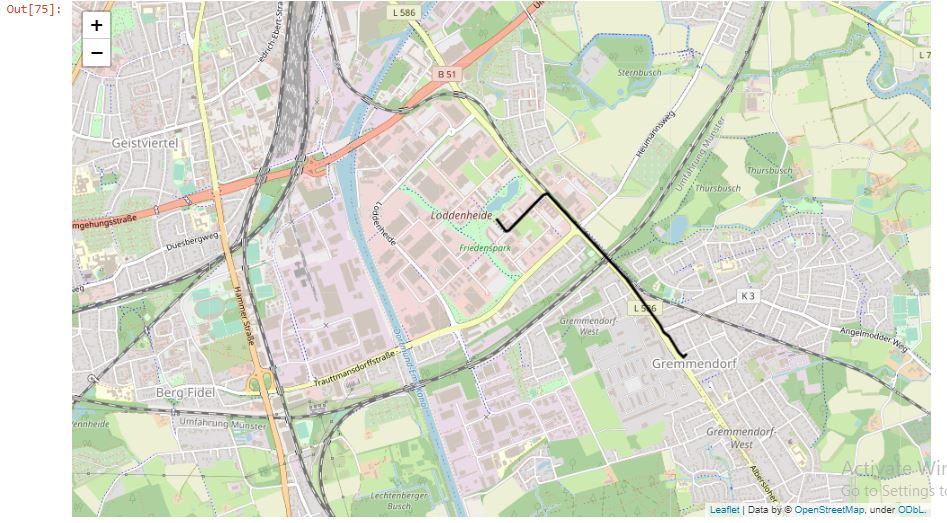
\includegraphics[width=1\linewidth,height=10cm]{folium.jpg} 
		\caption{Visualization using folium}
		\label{fig:workflow}
	\end{figure}
\end{tcolorbox}
        
    \hypertarget{example-visualization-with-pydeck-deck.gl}{%
\section{Example: Visualization with pydeck
(deck.gl)}\label{example-visualization-with-pydeck-deck.gl}}

    The pydeck library makes use of the basemap tiles from Mapbox. In case
you want to visualize the map with basemap tiles, you need to register
with MapBox, and configure a specific access token. The service is free
until a certain level of traffic is esceeded.

You can either configure it via your terminal (i.e.
\texttt{export\ MAPBOX\_API\_KEY=\textless{}mapbox-key-here\textgreater{}}),
which pydeck will automatically read, or you can pass it as a variable
to the generation of pydeck (i.e.
\texttt{pdk.Deck(mapbox\_key=\textless{}mapbox-key-here\textgreater{},\ ...)}.

    \begin{tcolorbox}[breakable, size=fbox, boxrule=1pt, pad at break*=1mm,colback=cellbackground, colframe=cellborder]
\prompt{In}{incolor}{83}{\boxspacing}
\begin{Verbatim}[commandchars=\\\{\}]
\PY{k+kn}{import} \PY{n+nn}{pydeck} \PY{k}{as} \PY{n+nn}{pdk}

\PY{c+c1}{\PYZsh{} for pydeck the attributes have to be flat}
\PY{n}{track\PYZus{}df}\PY{p}{[}\PY{l+s+s1}{\PYZsq{}}\PY{l+s+s1}{lat}\PY{l+s+s1}{\PYZsq{}}\PY{p}{]} \PY{o}{=} \PY{n}{track\PYZus{}df}\PY{p}{[}\PY{l+s+s1}{\PYZsq{}}\PY{l+s+s1}{geometry}\PY{l+s+s1}{\PYZsq{}}\PY{p}{]}\PY{o}{.}\PY{n}{apply}\PY{p}{(}\PY{k}{lambda} \PY{n}{coord}\PY{p}{:} \PY{n}{coord}\PY{o}{.}\PY{n}{y}\PY{p}{)}
\PY{n}{track\PYZus{}df}\PY{p}{[}\PY{l+s+s1}{\PYZsq{}}\PY{l+s+s1}{lng}\PY{l+s+s1}{\PYZsq{}}\PY{p}{]} \PY{o}{=} \PY{n}{track\PYZus{}df}\PY{p}{[}\PY{l+s+s1}{\PYZsq{}}\PY{l+s+s1}{geometry}\PY{l+s+s1}{\PYZsq{}}\PY{p}{]}\PY{o}{.}\PY{n}{apply}\PY{p}{(}\PY{k}{lambda} \PY{n}{coord}\PY{p}{:} \PY{n}{coord}\PY{o}{.}\PY{n}{x}\PY{p}{)}
\PY{n}{vis\PYZus{}df} \PY{o}{=} \PY{n}{pd}\PY{o}{.}\PY{n}{DataFrame}\PY{p}{(}\PY{n}{track\PYZus{}df}\PY{p}{)}
\PY{n}{vis\PYZus{}df}\PY{p}{[}\PY{l+s+s1}{\PYZsq{}}\PY{l+s+s1}{speed}\PY{l+s+s1}{\PYZsq{}}\PY{p}{]} \PY{o}{=} \PY{n}{vis\PYZus{}df}\PY{p}{[}\PY{l+s+s1}{\PYZsq{}}\PY{l+s+s1}{GPS Speed.value}\PY{l+s+s1}{\PYZsq{}}\PY{p}{]}

\PY{c+c1}{\PYZsh{} omit unit columns}
\PY{n}{vis\PYZus{}df\PYZus{}cols} \PY{o}{=} \PY{p}{[}\PY{n}{col} \PY{k}{for} \PY{n}{col} \PY{o+ow}{in} \PY{n}{vis\PYZus{}df}\PY{o}{.}\PY{n}{columns} \PY{k}{if} \PY{n}{col}\PY{o}{.}\PY{n}{lower}\PY{p}{(}\PY{p}{)}\PY{p}{[}\PY{n+nb}{len}\PY{p}{(}\PY{n}{col}\PY{p}{)}\PY{o}{\PYZhy{}}\PY{l+m+mi}{4}\PY{p}{:}\PY{n+nb}{len}\PY{p}{(}\PY{n}{col}\PY{p}{)}\PY{p}{]} \PY{o}{!=} \PY{l+s+s1}{\PYZsq{}}\PY{l+s+s1}{unit}\PY{l+s+s1}{\PYZsq{}}\PY{p}{]}
\PY{n}{vis\PYZus{}df} \PY{o}{=} \PY{n}{vis\PYZus{}df}\PY{p}{[}\PY{n}{vis\PYZus{}df\PYZus{}cols}\PY{p}{]}

\PY{n}{layer} \PY{o}{=} \PY{n}{pdk}\PY{o}{.}\PY{n}{Layer}\PY{p}{(}
    \PY{l+s+s1}{\PYZsq{}}\PY{l+s+s1}{ScatterplotLayer}\PY{l+s+s1}{\PYZsq{}}\PY{p}{,}
    \PY{n}{data}\PY{o}{=}\PY{n}{vis\PYZus{}df}\PY{p}{,}
    \PY{n}{get\PYZus{}position}\PY{o}{=}\PY{l+s+s1}{\PYZsq{}}\PY{l+s+s1}{[lng, lat]}\PY{l+s+s1}{\PYZsq{}}\PY{p}{,}
    \PY{n}{auto\PYZus{}highlight}\PY{o}{=}\PY{k+kc}{True}\PY{p}{,}
    \PY{n}{get\PYZus{}radius}\PY{o}{=}\PY{l+m+mi}{10}\PY{p}{,}          \PY{c+c1}{\PYZsh{} Radius is given in meters}
    \PY{n}{get\PYZus{}fill\PYZus{}color}\PY{o}{=}\PY{l+s+s1}{\PYZsq{}}\PY{l+s+s1}{[speed \PYZlt{} 20 ? 0 : (speed \PYZhy{} 20)*8.5, speed \PYZlt{} 50 ? 255 : 255 \PYZhy{} (speed\PYZhy{}50)*8.5, 0, 140]}\PY{l+s+s1}{\PYZsq{}}\PY{p}{,}  \PY{c+c1}{\PYZsh{} Set an RGBA value for fill}
    \PY{n}{pickable}\PY{o}{=}\PY{k+kc}{True}
\PY{p}{)}

\PY{c+c1}{\PYZsh{} Set the viewport location}
\PY{n}{view\PYZus{}state} \PY{o}{=} \PY{n}{pdk}\PY{o}{.}\PY{n}{ViewState}\PY{p}{(}
    \PY{c+c1}{\PYZsh{}longitude=7.5963592529296875,}
    \PY{c+c1}{\PYZsh{}latitude=51.96246168188569,    \PYZsh{}7.65079 51.95400}
    \PY{n}{longitude}\PY{o}{=}\PY{l+m+mf}{7.65079}\PY{p}{,}
    \PY{n}{latitude}\PY{o}{=}\PY{l+m+mf}{51.95400}\PY{p}{,}
    \PY{n}{zoom}\PY{o}{=}\PY{l+m+mi}{13}\PY{p}{,}
    \PY{n}{min\PYZus{}zoom}\PY{o}{=}\PY{l+m+mi}{5}\PY{p}{,}
    \PY{n}{max\PYZus{}zoom}\PY{o}{=}\PY{l+m+mi}{18}\PY{p}{,}
    \PY{n}{pitch}\PY{o}{=}\PY{l+m+mf}{40.5}\PY{p}{,}
    \PY{n}{bearing}\PY{o}{=}\PY{o}{\PYZhy{}}\PY{l+m+mf}{27.36}\PY{p}{)}

\PY{n}{r} \PY{o}{=} \PY{n}{pdk}\PY{o}{.}\PY{n}{Deck}\PY{p}{(}
    \PY{n}{width}\PY{o}{=}\PY{l+m+mi}{200}\PY{p}{,} 
    \PY{n}{layers}\PY{o}{=}\PY{p}{[}\PY{n}{layer}\PY{p}{]}\PY{p}{,} 
    \PY{n}{initial\PYZus{}view\PYZus{}state}\PY{o}{=}\PY{n}{view\PYZus{}state}\PY{p}{,} 
    \PY{n}{mapbox\PYZus{}key}\PY{o}{=}\PY{l+s+s2}{\PYZdq{}}\PY{l+s+s2}{pk.eyJ1IjoiamFuYWtwYXJhanVsaSIsImEiOiJjaWdtMWd2eWUwMjRvdXJrcjVhbTFvcmszIn0.jRIRtmgCm5waI7RXih3t5A}\PY{l+s+s2}{\PYZdq{}}
\PY{p}{)}
\PY{n}{r}\PY{o}{.}\PY{n}{to\PYZus{}html}\PY{p}{(}\PY{l+s+s1}{\PYZsq{}}\PY{l+s+s1}{tracks\PYZus{}muenster.html}\PY{l+s+s1}{\PYZsq{}}\PY{p}{,} \PY{n}{iframe\PYZus{}width}\PY{o}{=}\PY{l+m+mi}{900}\PY{p}{,} \PY{n}{iframe\PYZus{}height} \PY{o}{=} \PY{l+m+mi}{500}\PY{p}{)}
\end{Verbatim}
\end{tcolorbox}

    
    \begin{verbatim}
<IPython.lib.display.IFrame at 0x23dfa425ec8>
    \end{verbatim}

    
            \begin{tcolorbox}[breakable, size=fbox, boxrule=.5pt, pad at break*=1mm, opacityfill=0]
\prompt{Out}{outcolor}{83}{\boxspacing}
\begin{Verbatim}[commandchars=\\\{\}]
'D:\textbackslash{}\textbackslash{}MSC\_GeoTech\textbackslash{}\textbackslash{}Study\_Materials\textbackslash{}\textbackslash{}Course\textbackslash{}\textbackslash{}Second\_Semester\textbackslash{}\textbackslash{}Floating\_Car\_Project
\textbackslash{}\textbackslash{}enviroCar\textbackslash{}\textbackslash{}envirocar-py\textbackslash{}\textbackslash{}examples\textbackslash{}\textbackslash{}tracks\_muenster.html'
\end{Verbatim}
\end{tcolorbox}
        
\textbf{Brief description of your experience:- what went fine, where did you
face problems and how did you overcome the problems?}

    My start of the assignment had to pay a lot of toil in installing the software and its packages. I installed Anaconda3 with ease and then tried to install the packages and dependencies for geopandas and envirocar. Even both of them were installed and shown by the command 'conda list' in anaconda powershell prompt, a problem called 'ModuleImportError' would show whenever I tried to import the modules in Python terminal. I had to uninstall and reinstall the Anaconda software a lot of times before figuring out the problem. I uninstalled all other previously installed Python3, deleted its environment settings and removed from the registry editor also. I also uninstalled previously installed osgeo and removed gdal settings. Then, I had to manually install the wheel files of the dependencies of geopandas (GDAL, Fiona, Pyproj, Rtree and Shapely) from a repository maintained by \href{https://www.lfd.uci.edu/~gohlke/pythonlibs/}{Christoph Gohlke at the Laboratory for Fluorescence Dynamics at UC Irvine} . The steps followed was from this link: \href{https://geoffboeing.com/2014/09/using-geopandas-windows/?fbclid=IwAR1c1qrPEm0QmVnvl4drel7aZ\_pU\_Bh\_QN-1Z8QxzhY0RNBWXeApJpBVZ-Y}{Geoffboeing} .

    Upon completion of the detailed instructions given in the link above, finally geopandas was successfully installed and imported. Then, envirocar package was successfully installed using the command 'pip install envirocar-py --upgrade'. It took more than two full days to figure it and sort out the problem. 
    Happily, no further problems were faced in course of modification of the given project.


\textbf{Screenprint(s) of the last page of the Notebook, presenting the
result of your modification..}

    \begin{tcolorbox}[breakable, size=fbox, boxrule=1pt, pad at break*=1mm,colback=cellbackground, colframe=cellborder]
\prompt{In}{incolor}{ }{\boxspacing}
\begin{figure}[H]
	\centering
	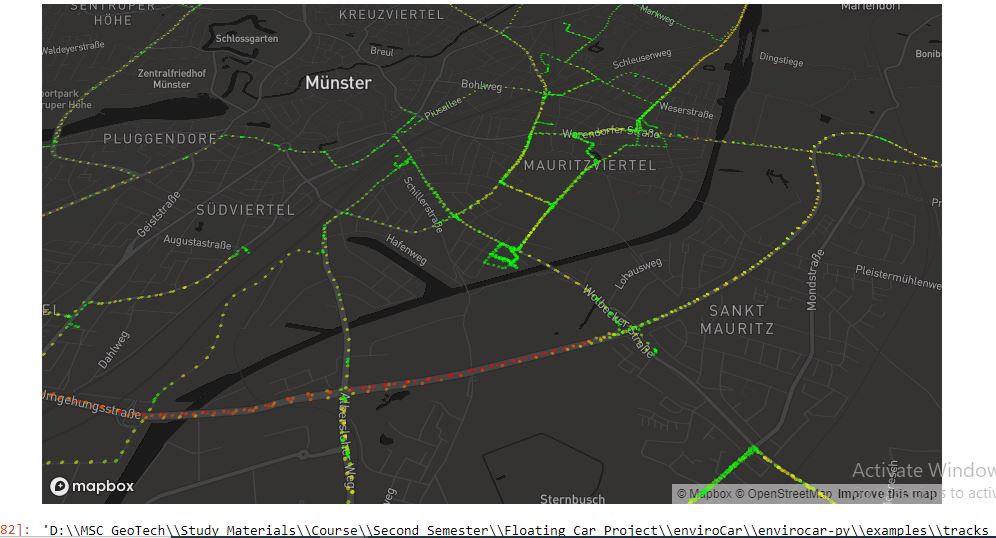
\includegraphics[width=1\linewidth,height=10cm]{pydeck.jpg} 
	\caption{Visualization with pydeck}
	\label{fig:workflow}
\end{figure}
\begin{Verbatim}[commandchars=\\\{\}]

\end{Verbatim}
\end{tcolorbox}


    % Add a bibliography block to the postdoc
    
    
    
\end{document}
